\documentclass[12pt,a4paper]{report}
\usepackage{graphicx,iman,extra,ttbox,pdfsetup}

\title{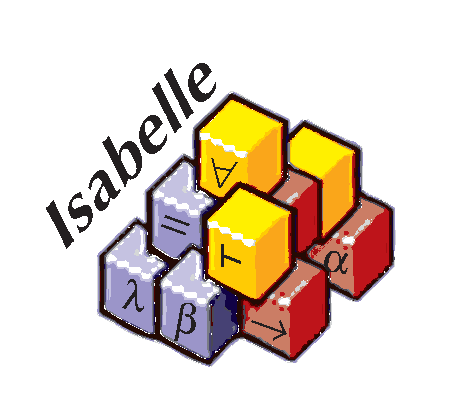
\includegraphics[scale=0.5]{isabelle} \\[4ex] Old Isabelle Reference Manual}

\author{{\em Lawrence C. Paulson}\\
        Computer Laboratory \\ University of Cambridge \\
        \texttt{lcp@cl.cam.ac.uk}\\[3ex] 
        With Contributions by Tobias Nipkow and Markus Wenzel}  

\setcounter{secnumdepth}{2} \setcounter{tocdepth}{2}

\pagestyle{headings}
\sloppy
\binperiod     %%%treat . like a binary operator

\begin{document}
\underscoreoff

\index{definitions|see{rewriting, meta-level}}
\index{rewriting!object-level|see{simplification}}
\index{meta-rules|see{meta-rules}}

\maketitle 
\emph{Note}: this document is part of the earlier Isabelle
documentation and is mostly outdated.  Fully obsolete parts of the
original text have already been removed.  The remaining material
covers some aspects that did not make it into the newer manuals yet
\cite{isabelle-isar-ref,isabelle-implementation}.

\subsubsection*{Acknowledgements} 
Tobias Nipkow, of T. U. Munich, wrote most of
  Chapters~\protect\ref{Defining-Logics} and~\protect\ref{chap:simplification}.
  Markus Wenzel contributed to Chapter~\protect\ref{chap:syntax}.
  Jeremy Dawson, Sara Kalvala, Martin
  Simons  and others suggested changes
  and corrections.  The research has been funded by the EPSRC (grants
  GR/G53279, GR/H40570, GR/K57381, GR/K77051, GR/M75440) and by ESPRIT
  (projects 3245: Logical Frameworks, and 6453: Types), and by the DFG
  Schwerpunktprogramm \emph{Deduktion}.

\pagenumbering{roman} \tableofcontents \clearfirst

%%seealso's must be last so that they appear last in the index entries
\index{meta-rewriting|seealso{tactics, theorems}}

\begingroup
  \bibliographystyle{plain} \small\raggedright\frenchspacing
  \bibliography{manual}
\endgroup

\end{document}
